%========= Introduction
\section{Introduction}
\label{sec:introduction}

In the complex and ever-evolving world of \ac{EW}, quantum computing could provide the ability to understand radar signals in novel ways, never before seen in this field. 
It is widely recognised in the discipline of electronic warfare that traditional signal analysis techniques are still bounded by computational constraints, so in order to maintain strategic advantage, new techniques are continuously needed in order to keep pace with emerging threats. 
Quantum computing may promise a paradigmatic shift in extracting actionable insights from massive and complex \ac{EW} datasets. 

Recent research has demonstrated a great potential for quantum computing to address the challenges of modern signal processing \cite{somma_quantum_2019, daskin_walk_2022},
however little work has been devoted to its applications in \ac{EW} signal processing, and more specifically radar signal processing.
Therefore, this report explores the question of how quantum technology may be applied to radar signal processing in \ac{EW}.
At first, a survey of the current state of research will be conducted for radar signal analysis and quantum signal processing. 
Then, an empirical enquiry into the subject will be presented, aiming to determine how quantum methods can be used to encode, detect, and characterise radar signals.
Finally, a discussion of results, examination of limitations, and consideration for future work will be provided. 

Despite quantum computing holding much promise, its potential in this field remains largely unexplored.
This report presents a background and preliminary investigation into how quantum computing might be utilised in the dynamic landscape of electronic warfare. 

\subsection{Background}~\label{subsec:background}

%% Definition
The electromagnetic environment is akin to a bustling city street, teeming with unrelenting noise and countless signals that evade human perception.
In modern-day warfare, this invisible domain is critical, and it takes specialised tools and techniques to make sense of the chaos.
\ac{ESM} attempts to understand this situation, enabling operators to extract valuable intelligence from the cacophonous electromagnetic environment.
Put simply, the goal is to identify and locate potential threats using information from the spectrum.
Despite engineers and operators developing advanced tools and techniques to overcome the challenges posed by this crowded environment, the inherent complexity and current technology constraints mean that \ac{ESM} remains a mostly unsolved problem.

Among the countless signals that \ac{ESM} operators must sift through, radar signals are of particular interest due to their widespread use in military and civilian contexts.
Since radar's invention in 1930 \cite{degering_invention_2018}, it has been an invaluable tool for making the invisible visible.
It is "an electrical system that transmits \ac{RF} electromagnetic waves toward a region of interest and receives and detects these EM waves when reflected from objects in that region."\cite{richards_principles_2010}.
Radar probes the environment to detect any potential impediments or hazards, and it is those probes that \ac{ESM} systems aim to intercept and understand.

%% History
% Etymological
The name radar originates from a portmanteau of \textit{Radio Detection and Ranging}\cite{the_joint_board_on_scientific_information_policy_radar_1945}, hinting at it's founding objectives in the defence context. In the modern day, radar is used in many applications \cite{merrill_i_skolnik_radar_nodate, desai_how_2022}, including:
\begin{itemize}
    \item Aerospace - weather, navigation, approach, altitude, identification
    \item Maritime - navigation, collision avoidance,  
    \item Ground Penetrating - archaeology, mining, oceanographic sounding
    \item Space - spacecraft and celestial monitoring
    \item Automotive - civilian and law enforcement
    \item Industrial - fluid sensing, speed measurement
    \item Atmospheric - meteorological, gas concentration measurements
    \item Electronic Warfare - direction finding, jamming, \ac{ELINT}
\end{itemize}

% Consequence: dense + interference
As a result, the electromagnetic environment has become increasingly densely populated, with a multitude of different emitters competing for spectrum space (not to mention other challenges such as shadowing, clutter and other sources of natural or intentional interference)
% Oppurtunity
However, due to their widespread adoption - particularly in the defence context - an opportunity arises: potentially being able to identify and locate any military target with an \ac{RF} emission.
% Over-arching goal
\begin{figure}
    \centering
    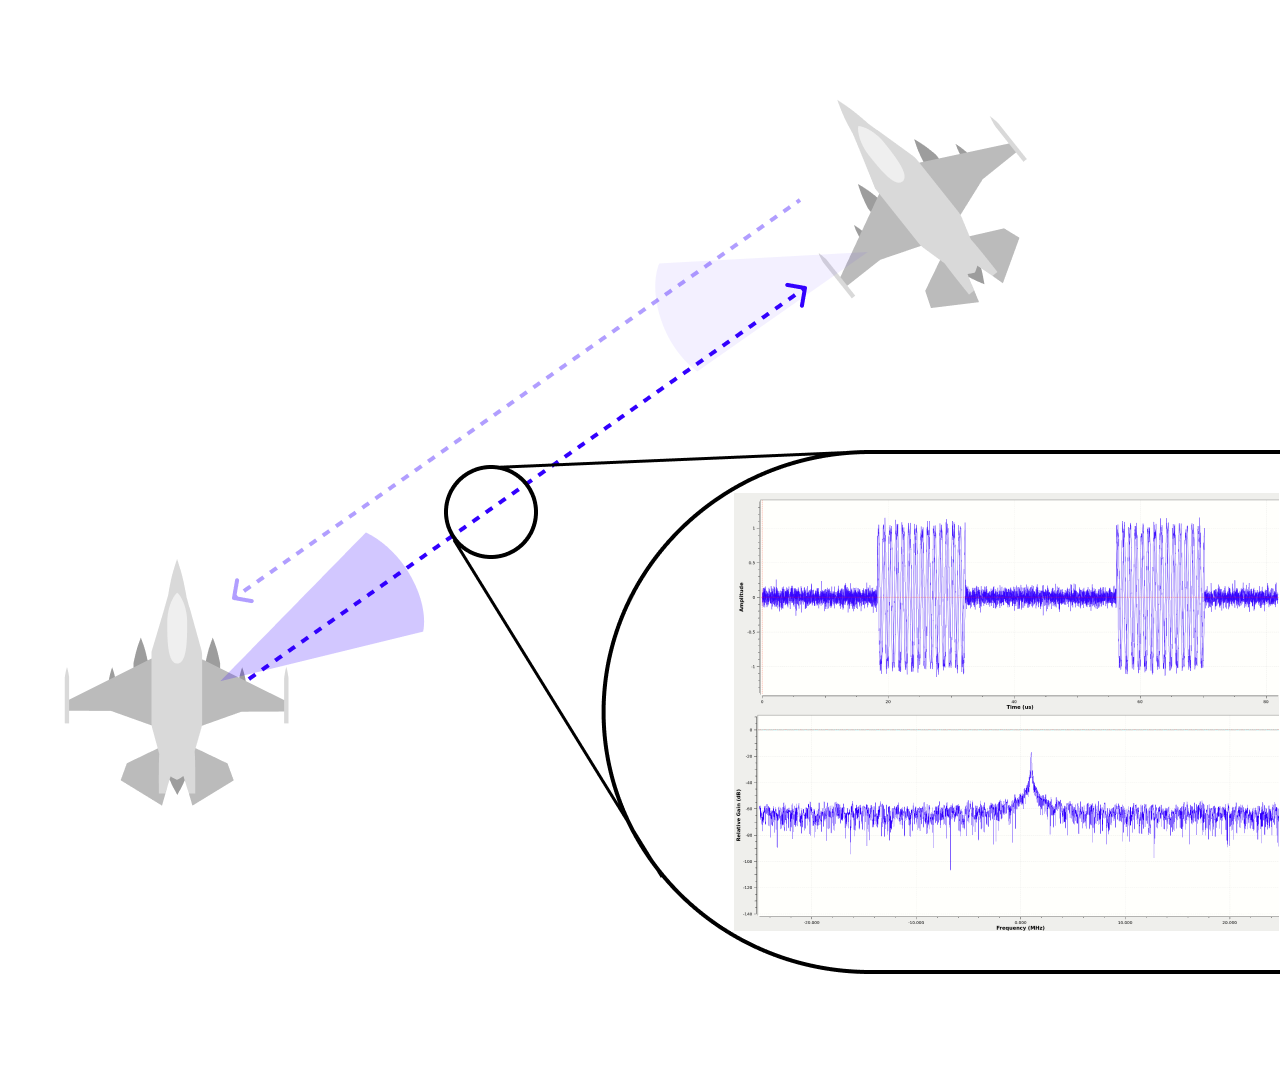
\includegraphics[width=0.9\textwidth]{Figures/Senario_ Single Radar; single signal.png}
    \caption{Simplified situation for radar use in ESM.}
    \label{Fig:radar_signals_in_ew}
\end{figure}

While a difficult (and probably impossible) objective, it is the ideal goal of any \ac{ESM} system (see Figure \ref{Fig:radar_signals_in_ew}).

A more formal definition of this subject has been given by D. Adamy \cite{adamy_13_2001} as: \ac{EW} being "the art and science of preserving the use of the electromagnetic spectrum for friendly use while denying its use to the enemy", and \ac{ESM} being "the receiving part of EW" \cite{adamy_13_2001}, of which radar is the principal element.

\todo{Principles of radar}

% A typical radar system is made up of at least one of each: radio transmitter, radio receiver, antenna, and display \cite{stimson_introduction_1998}. % There was a more precise definition somewhere with a 'signal processor' element.

% The ESM pipeline
% ------------

% ------------------------------

For the radar to achieve its objectives, it must be able to convert observed data into actionable information, thereby requiring some degree of information processing. 
Herein lies the general functions in \ac{ESM} - the detection, location, and identification of targets, which will now be explored. % Cite 'detection, location and identification' - I think the precise term is 'analysis'.

First, however, a conceptual schematisation of this system must be made in in terms of its inputs, process, and outputs. In \ac{ESM}, inputs consist of EM fluctuations that vary over time. They are almost always received by an antenna (or antennas) which may be subsequently manipulated in the analogue and digital domains. These fluctuations, henceforth \textit{signals} (not to be confused with communications signals), are the essential information carriers in the signal processing operation. There also exist inputs derived from the nature of the radar system configuration itself. These may include the antenna configuration and receiver architecture which will not here be considered, but is noted by the author as being of significant relevance to kinematic measurement and capability constraints.

Since the signals of interest are those emitted by radar systems, the received signals exhibit phenomenal qualities corresponding to those of the originating radar, featuring a number of characteristic parameters \cite[sect. 5-8.1]{avionics_department_electronic_2013}: 
\begin{itemize}
    \item Frequency (\ac{RF}): Intrapulse frequency, modulation (and associated modulation parameters); Interpulse: phase coherence.
    \item Amplitude (power)
    \item \ac{DOA} / \ac{AOA}
    \item \ac{TOA}
    \item \ac{PRI} / \ac{PRF}
    \item \ac{PRI} type
    \item \ac{PW}
    \item Scan type and rate
    \item Lobe duration (beam width or dwell)
\end{itemize}

Figure \ref{fig:pulse_train} provides an example of a pulse train with a number of its parameters highlighted and annotated.

\begin{figure}[t]
    \centering
    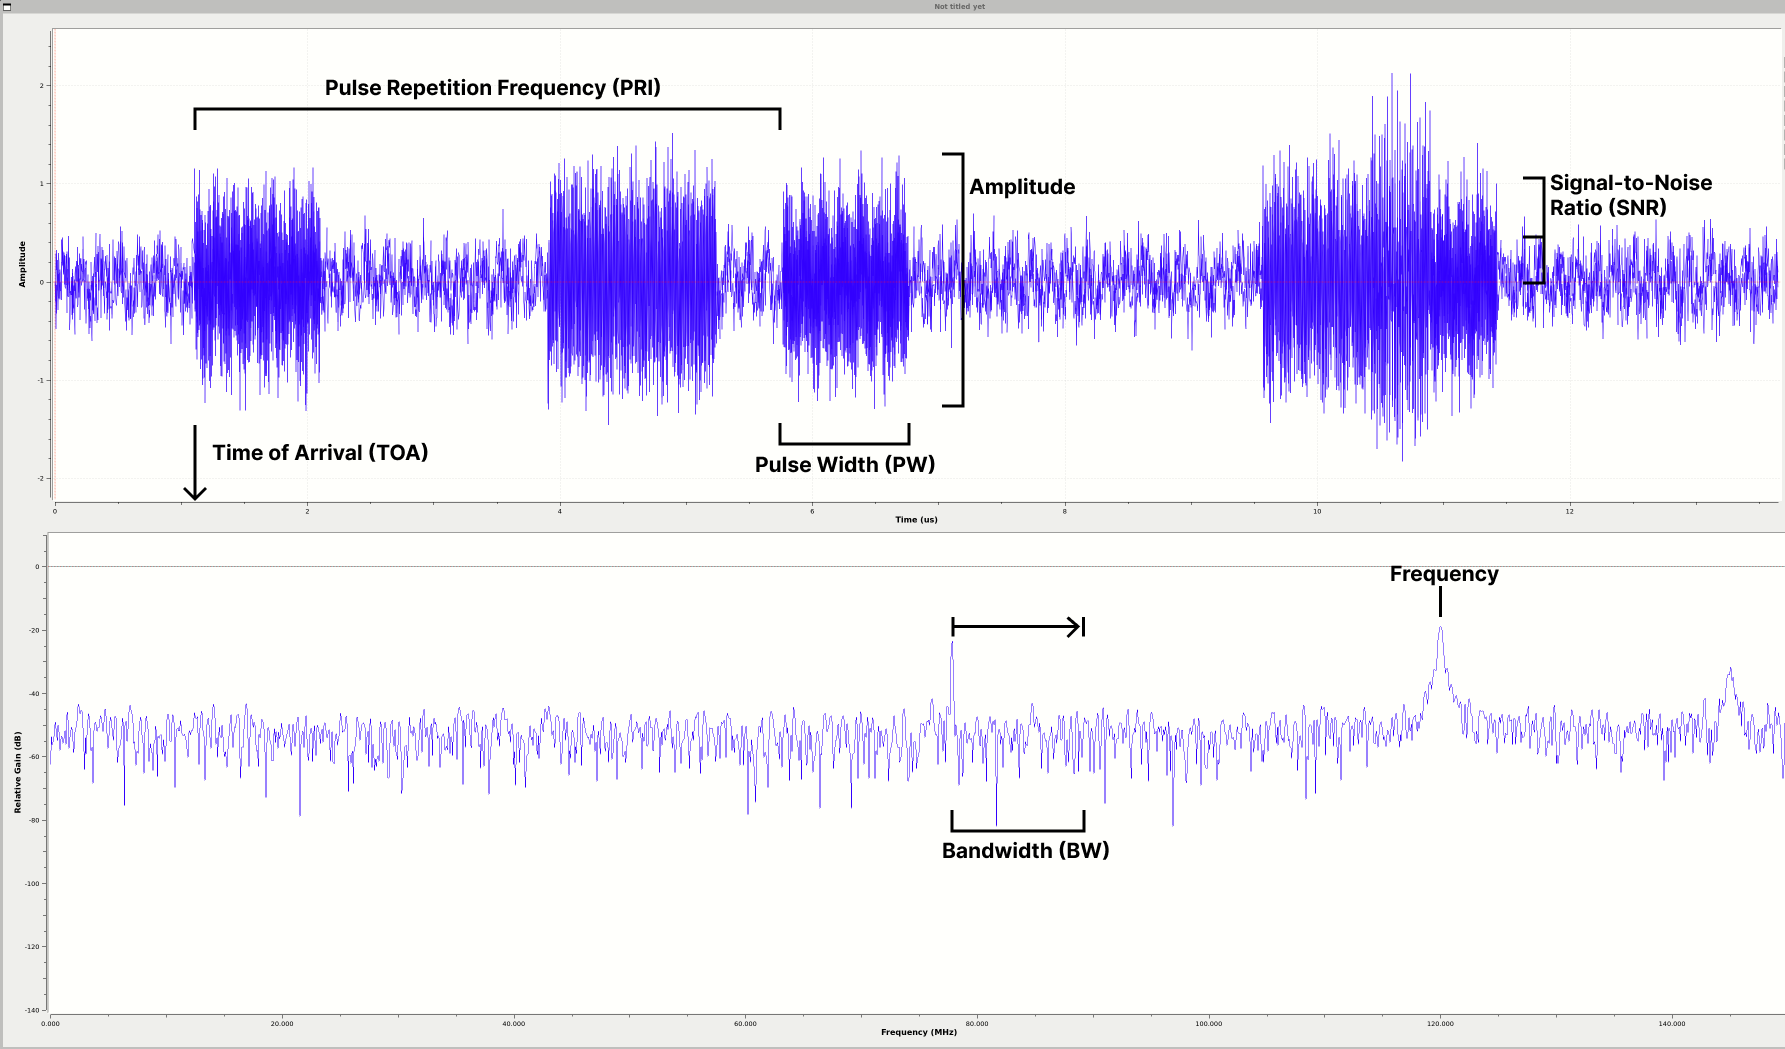
\includegraphics[width=1\textwidth]{Figures/annotated.png}
    \caption{Pulse train, annotated with signal parameters}
    \label{fig:pulse_train}
\end{figure}

The role of the processing step, is to convert the 'raw' signal into these parameters, which, ideally should correspond to those nominally transmitted by the target radar.
Parameters are generally extracted from the incident \ac{EM} signals and may be treated independently as outputs themselves. Typically, however, further analysis may be may conducted to yield more granular and actionable information. Information that \ac{ESM} seeks to understand addresses many facets:
\begin{itemize}
    \item Target detection
    \item Target characteristics \cite{jenn_radar_2007}
    \begin{itemize}
        \item target size - return amplitude
        \item target shape - from discrete scan returns
        \item target material composition
        \item moving parts (modulation of the return)
    \end{itemize}
    \item Target identification
    \item Kinematic parameters and tracking(range, direction, speed, \ac{AOA})
\end{itemize}

% extract
After having digitised the radar signals, the signal processing process then involves extracting meaningful information from the signals. 
% detect
In the context of the \ac{ESM} pipeline, various methods are used to detect radar pulses from a pulse train. 
Classically, this can be done using amplitude thresholding, or in more modern \ac{ESM} systems - neural networks \cite{liu_classification_2019, alhashimi_deinterleaving_2007}.
% pulse train
As seen in Figure \ref{fig:pulse_train}, there may be multiple, potentially overlapping pulses.
% parameter estimation
The detected pulses are then analysed to extract the characteristic parameters, or a \ac{PDW}.
Usually traditional signal processing techniques such as Fourier- or wavelet-transforms \cite{ehara_weak_1994, gulum_parameter_2012}
% ID
\ac{PDW}'s may then be associated with specific radar modes which can consequentially provide an indication of a known radar type.
This too is classically achieved using Bayesian methods \cite{matuszewski_knowledge-based_2008} and expert systems \cite{miah_expert_1999}
% Track
In parallel with this, a track of the target may be plotted for the radar operator.
% More analysis.
There are of course, many analysis additional steps to characterise, identify, and classify targets, not to mention the final decision-making processes \cite{charlish_development_2020}.

% constrained
Importantly, these methods are often bounded by computational constraints.
% why constrained
Despite significant advancements in signal processing and machine learning techniques, the sheer volume and complexity of the data from radar signals pose a challenge for traditional computing architectures.
% quantum?? there is precedent
It is therefore that quantum methods present a tentative solution, given that it is believed that it has the potential to solve certain NP-hard problems significantly faster than classical computers.
% developed
In recent years, researchers have made significant progress in developing quantum algorithms for signal processing applications.
% basic (QFT <=> Fourier transform)
For example, a basic quantum building-block - \ac{QFT}'s have shown the ability to automatically compute the Fourier transform, which is often used in \ac{ESM} analysis for extracting the frequency components of radar signals.
% moreequivilents
Some more complex classical analysis techniques have even been found to have direct quantum equivalents \cite{hoyer_efficient_1997, ma_quantum_2021, fijany_quantum_1998, nimbe_models_2021}.
% ML
The current state-of-the-art of \ac{EW} lies in applying novel \ac{ML} and \ac{AI} methods to all aspects of the discipline.
% quantum computing has an answer to that too!
Quantum computing in the context of hybrid quantum-classical machine learning has also been given significant research \cite{sim_expressibility_2019, schuld_quest_2014}.

% quantum is limited
However, quantum methods certainly have drawbacks, primarily due to its infancy and limited physical quantum hardware.
% NISQ .
In the current \ac{NISQ} era of quantum computing, practical methods are usually unsatisfactory.
% Early research 
However, with early research such as this, it is possible that real-world implementations may soon yield advantages in the defense context.

% conclusion
Nonetheless, given its large potential and potential suitability, quantum computing for \ac{ESM} signal analysis emerges as a logical next step in exploring a new frontier of \ac{EW} signal processing.

\subsubsection{Research Question}
How can quantum computing methods be used to in an \ac{ESM} function to detect the types and characteristics of radar signals in the defence context?

\subsubsection{Research Objectives}
\begin{enumerate}[label=Obj. \arabic*]
    \item Gain access to radar data that can be used to test and verify quantum implementations
    \item Implement a selection of quantum-based encoding techniques that convert sampled time-domain radar signals into the quantum domain.
    \item Produce an objective evaluation and validation of the quantum encoding methods by measuring the expressivity, complexity, and qualitative suitability.
    \item Develop a method for quantum-based pulse detection of a radar signals
    \item Present a quantitative evaluation of accuracy and signal-to-noise tolerance of the pulse detection method, for signals that vary in type and quality.
    \item Develop a method for quantum-based estimation of a radar signal's frequency.
    \item Present a quantitative evaluation of the accuracy and signal-to-noise tolerance of the frequency estimation method, for varying signals.
\end{enumerate}

\subsection{Scope}

The following list outlines the areas and topics that are outside the scope of this study:

\begin{itemize}
    \item Hardware - neither the physical implementation's of quantum nor radar will be considered.
    \item \ac{ESM}-focused. Only digitised signals to parameter estimation will be examined. Anything down-stream of identification of radar signals, (e.g., display, databasing, data fusion, etc.) and before digitisation (receive path, antennas, etc.) will be excluded
    \item \ac{SAR} and imaging radar functions
    \item Kinetic and located radar systems:
    \begin{itemize}
        \item Multi-path effects
        \item Located antennas - bi-static/multi-static; antenna arrays
        \item Range, velocity, angle of arrival, etc.
    \end{itemize}
    \item Radar emission. Only passive, or pure \ac{ESM} scenarios will be considered
    \item Detailed radar simulation will be excluded.
    \item The frequency range of interest considered will fall within \(50MHz - 1GHz\) and be exclusive of non-radar signals.
    \item Adjacent problems in radar will be granted only limited attention:
    \begin{itemize}
        \item Resource allocation
        \item Ambiguity analysis
        \item Tracking
    \end{itemize}
\end{itemize}

% --------------
% OLD OBJECTIVES
% --------------
% In the processing functional block, the problems for radar are, in sequential order:
% \begin{itemize}
%     \item How to distinguish between the different categories of signals: communications, interference, radar, and noise.
%     \item Then, after having understood what signals are radar intercepts, identifying which belong to the same originating receiver. 
%     \item Once, a radar signal has been de-interleaved, how to identify the originating emitter, given some a priori understanding of the operational environment.
% \end{itemize}
% \begin{itemize}
%     \item To further understand the principles of operation of passive radar systems, including their ability to detect and identify emitters in complex electromagnetic environments.
%     \item To critically evaluate existing literature on radar systems and quantum computing to effecively communicate existing the academic knowledge, and to show a capability to conduct independent future research.
%     \item To identify the possibilities of using Quantum Computing in Radar signal analysis; to also identify three candidate avenues; to explore one in enough depth to evaluate potential feasability though the creation of a technical solution
%     \item To prioritize research topics based on their level of desirability and feasibility, and to develop a plan for executing research projects within a defined timeline and scope.
%     \item To communicate research findings effectively to a technical audience.
% \end{itemize}
% \begin{itemize}
%     \item Identify a candidate method, or methods for converting continuously varying parameterised radar signals into into discrete radar modes using quantum methods?
%     \item Is it possible, and to what extent are quantum methods effective in de-interleaving and signal clustering?
%     \item Can quantum computing effectively track a radar signal intercept, and how well?
%     \item %\almarginpar{Would the last two-four be in too hard basket for the time frame? May be better to leave those for the motivation section - if we could do the previous then we'd be able to do the following?}
%     In the radar context, can, and how well are quantum computing methods disposed to help in reducing noise, interference, and clutter?
% \end{itemize}
